\documentclass[11pt, a4paper]{ltjsarticle}
\usepackage{amsmath}
\usepackage{amssymb}
\usepackage{bm}
\usepackage{graphicx}
\usepackage{luatexja}
\usepackage{fontspec}
\usepackage{geometry}
\usepackage{titlesec}
\usepackage{fancyhdr}
\usepackage{lastpage}
\usepackage{abstract}
\usepackage{datetime}
\setmainfont{IPAexMincho}
\setsansfont{IPAexGothic}
\setmonofont{IPAGothic}
\geometry{top=20mm, bottom=20mm, left=20mm, right=20mm}
\titleformat*{\section}{\large\bfseries}
\titleformat*{\subsection}{\normalsize\bfseries}
\titleformat*{\subsubsection}{\normalsize}
\pagestyle{fancy}
\fancyhf{}
\rhead{ページ \thepage/\pageref{LastPage}}
\lhead{知能情報論 最終課題}
\title{知能情報論 最終課題}
\author{37-246392  豊田 圭将}
\date{\the\year 年\,\the\month 月\, 2日}

\begin{document}

\maketitle

\section{はじめに}
本レポートでは、YouTubeの動画分析ツールの実装について説明する。このツールは、動画の情報取得、自動生成された字幕抽出、OCR処理、およびROUGE-Lスコアの計算と可視化を行うものである。

\section{実現した知的機械の概要と考えられる応用先}
本プロジェクトで実現した知的機械は、YouTubeの動画コンテンツを自動的に分析し、テキストデータの一致度を評価するシステムである。主な機能は動画のメタデータ収集、自動生成された字幕の抽出、動画フレームからのOCR処理、自動生成された字幕とOCR結果の比較分析、および分析結果の可視化である。

応用先としては、動画の字幕品質評価、コンテンツモデレーション、悪意のあるテキスト付き動画の検出などが挙げられる。

\section{利用した手法の説明}
本システムでは、以下の主要な手法を利用している:

\begin{itemize}
  \item YouTube Data API:動画のメタデータ取得
  \item YouTube Transcript API:自動生成された字幕の取得
  \item Google Cloud Vision API:OCR処理によるテキスト抽出
  \item ROUGE-L:自動生成された字幕とOCR結果のテキスト一致度評価
  \item 並列処理:ThreadPoolExecutorによる処理速度向上
\end{itemize}

\section{工夫した点の説明}
本システムの実装において、以下の点で独自の工夫を行った:

\begin{itemize}
  \item 動的なOCR処理範囲の決定:動画種類に応じてOCR処理領域を調整
  \item 適応的なOCR処理間隔:字幕のタイムスタンプに応じてフレームを抽出
  \item マルチスレッド処理の最適化:CPUコア数に応じて最適なスレッド数を決定
  \item エラー復旧メカニズム:指数バックオフアルゴリズムによる再試行
  \item チャンネル別分析機能:チャンネルごとのROUGE-Lスコア集計と比較分析
\end{itemize}

\section{利用した実データの説明}
本研究では、東京都知事選挙に関するYouTube動画500本(通常動画342本、ショート動画158本)を分析対象とした。通常動画では最初の5分間、ショート動画では1分間に対して処理を行った。

\section{得られた結果}
システムの実行結果から、以下の定量的評価と知見が得られた:

\subsection{ROUGE-Lスコアの分布}
\begin{itemize}
  \item 全動画の平均ROUGE-Lスコア:0.37
  \item 通常動画の平均ROUGE-Lスコア:0.36
  \item ショート動画の平均ROUGE-Lスコア:0.41
\end{itemize}

予想に反し、ショート動画の方が通常動画よりもROUGE-Lスコアが高い傾向が見られた。

\begin{figure}[htbp]
  \centering
  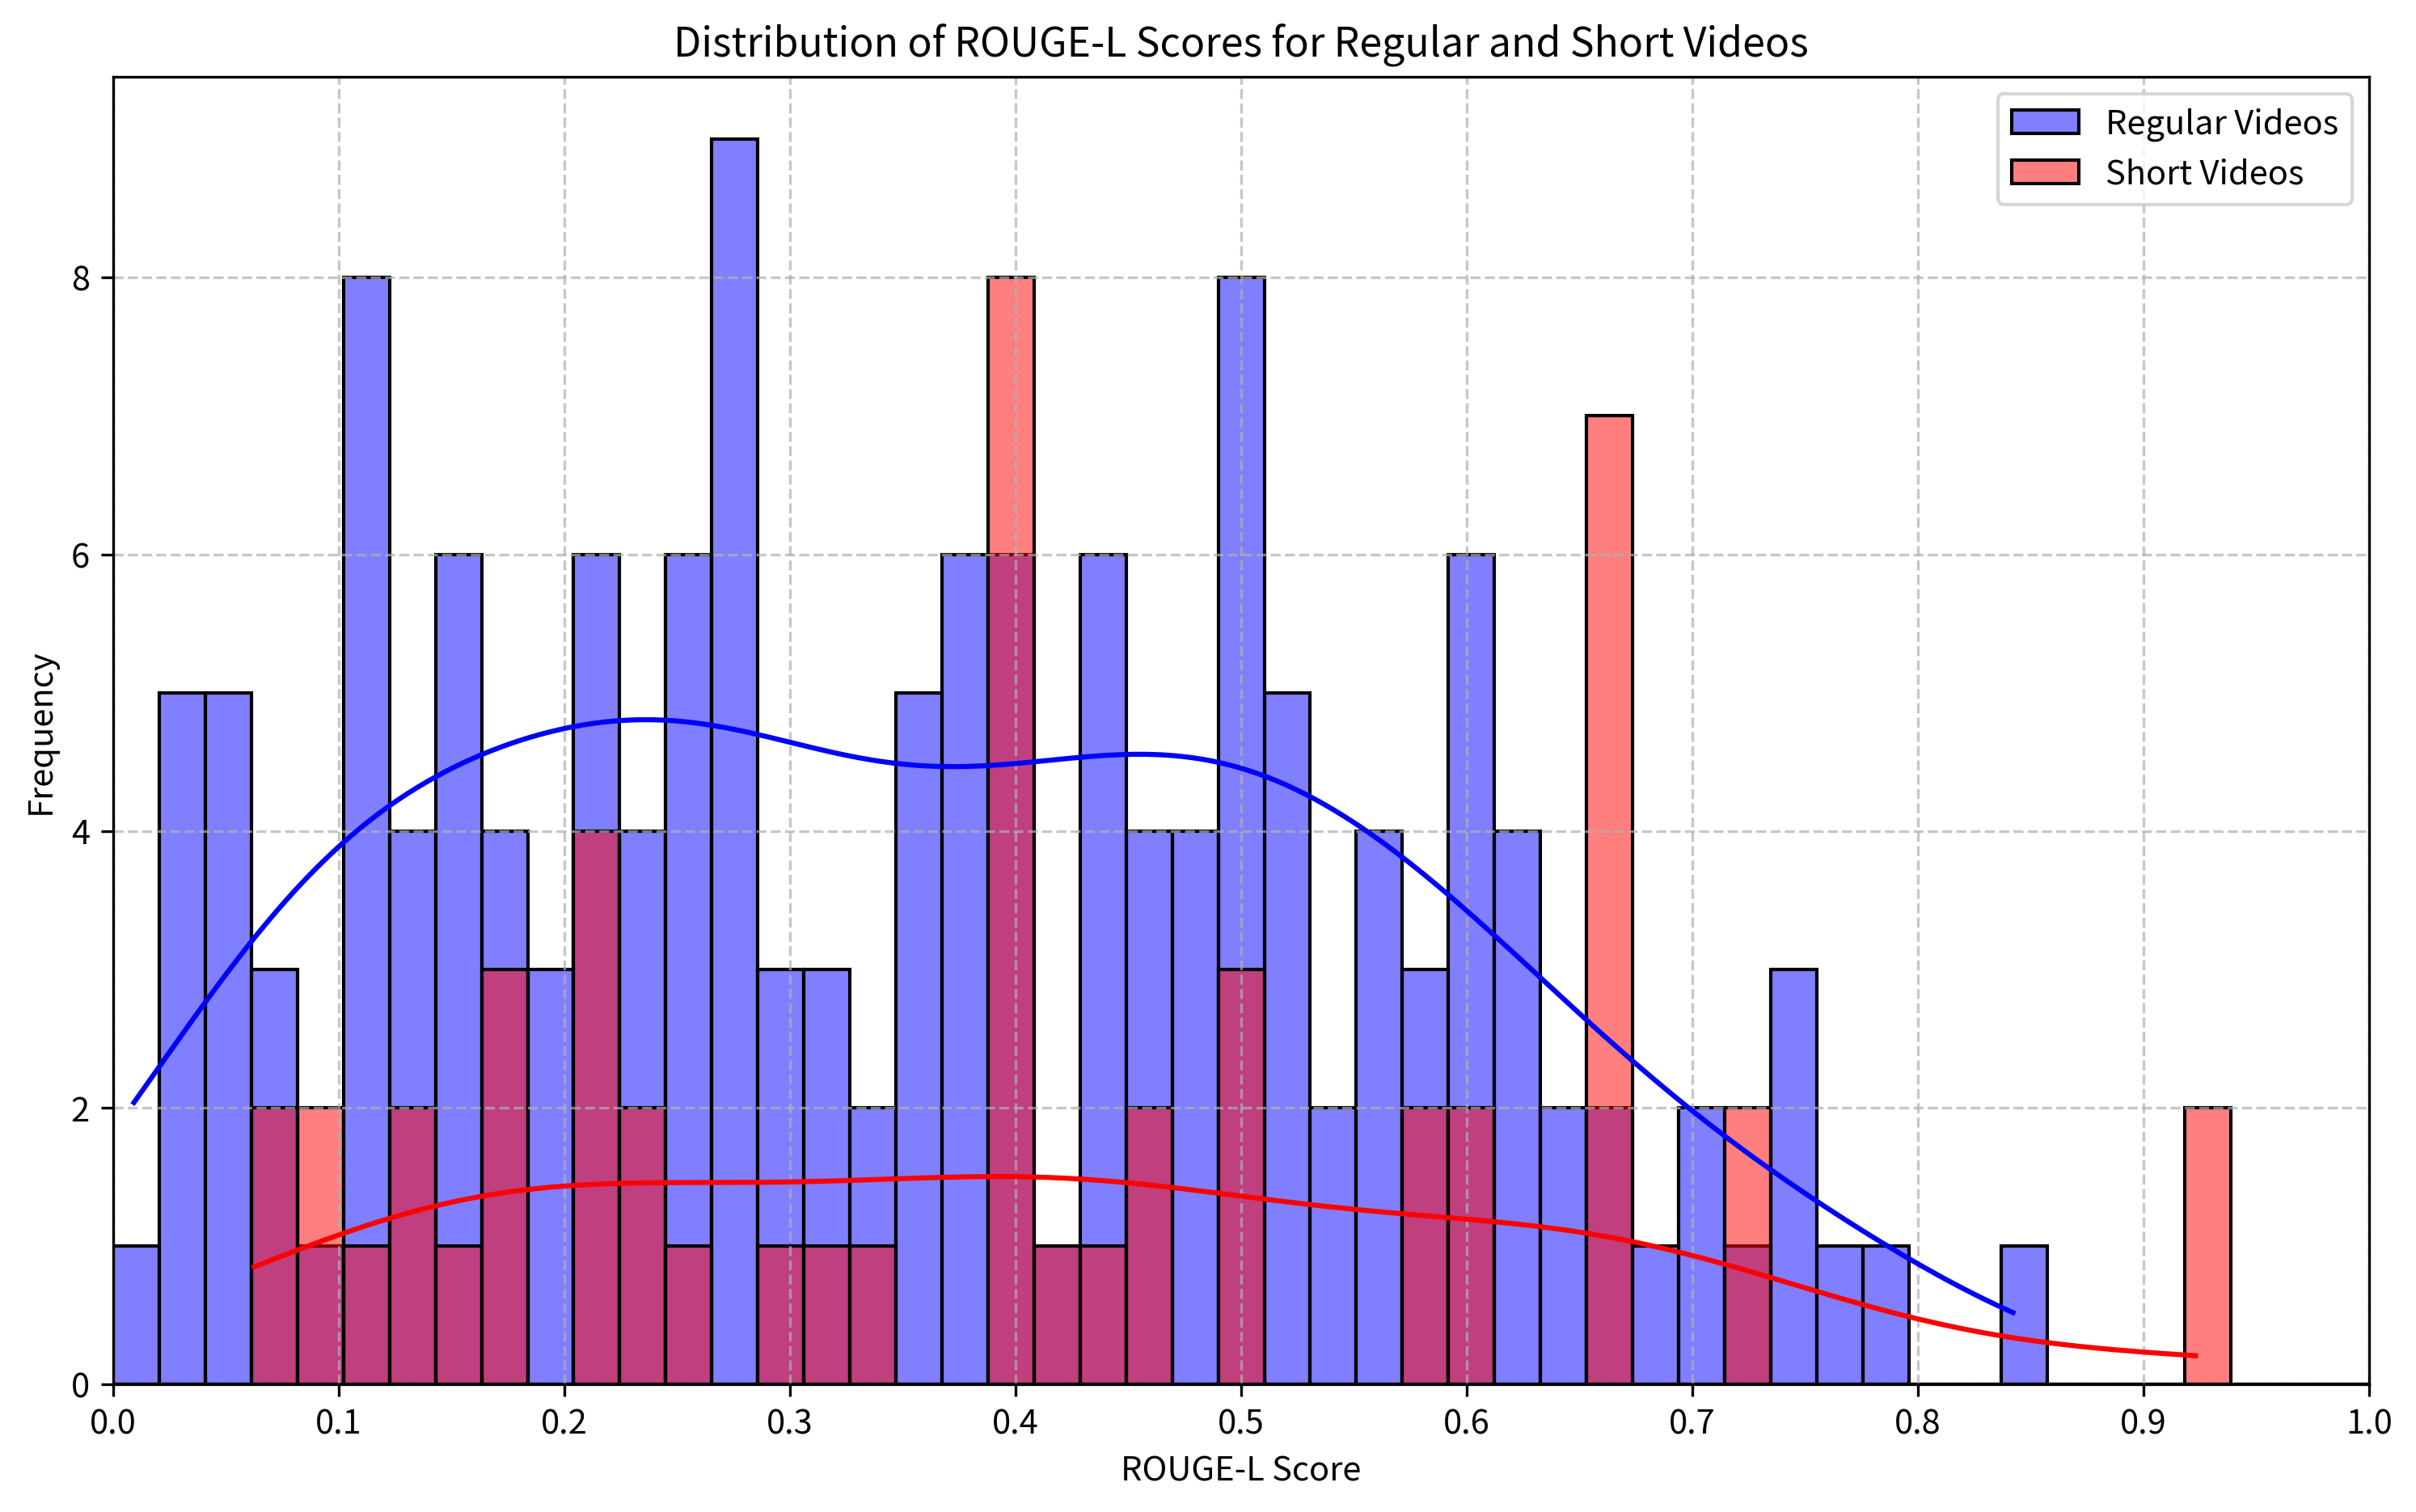
\includegraphics[width=0.65\textwidth]{../results/img/rouge_l_histogram_comparison.png}
  \caption{通常動画とショート動画のROUGE-Lスコア分布の比較}
\end{figure}

\subsection{再生回数とROUGE-Lスコアの相関}
再生回数とROUGE-Lスコアの間にはほとんど相関が見られなかった(Spearman's rank correlation:0.049)。

\begin{figure}[htbp]
  \centering
  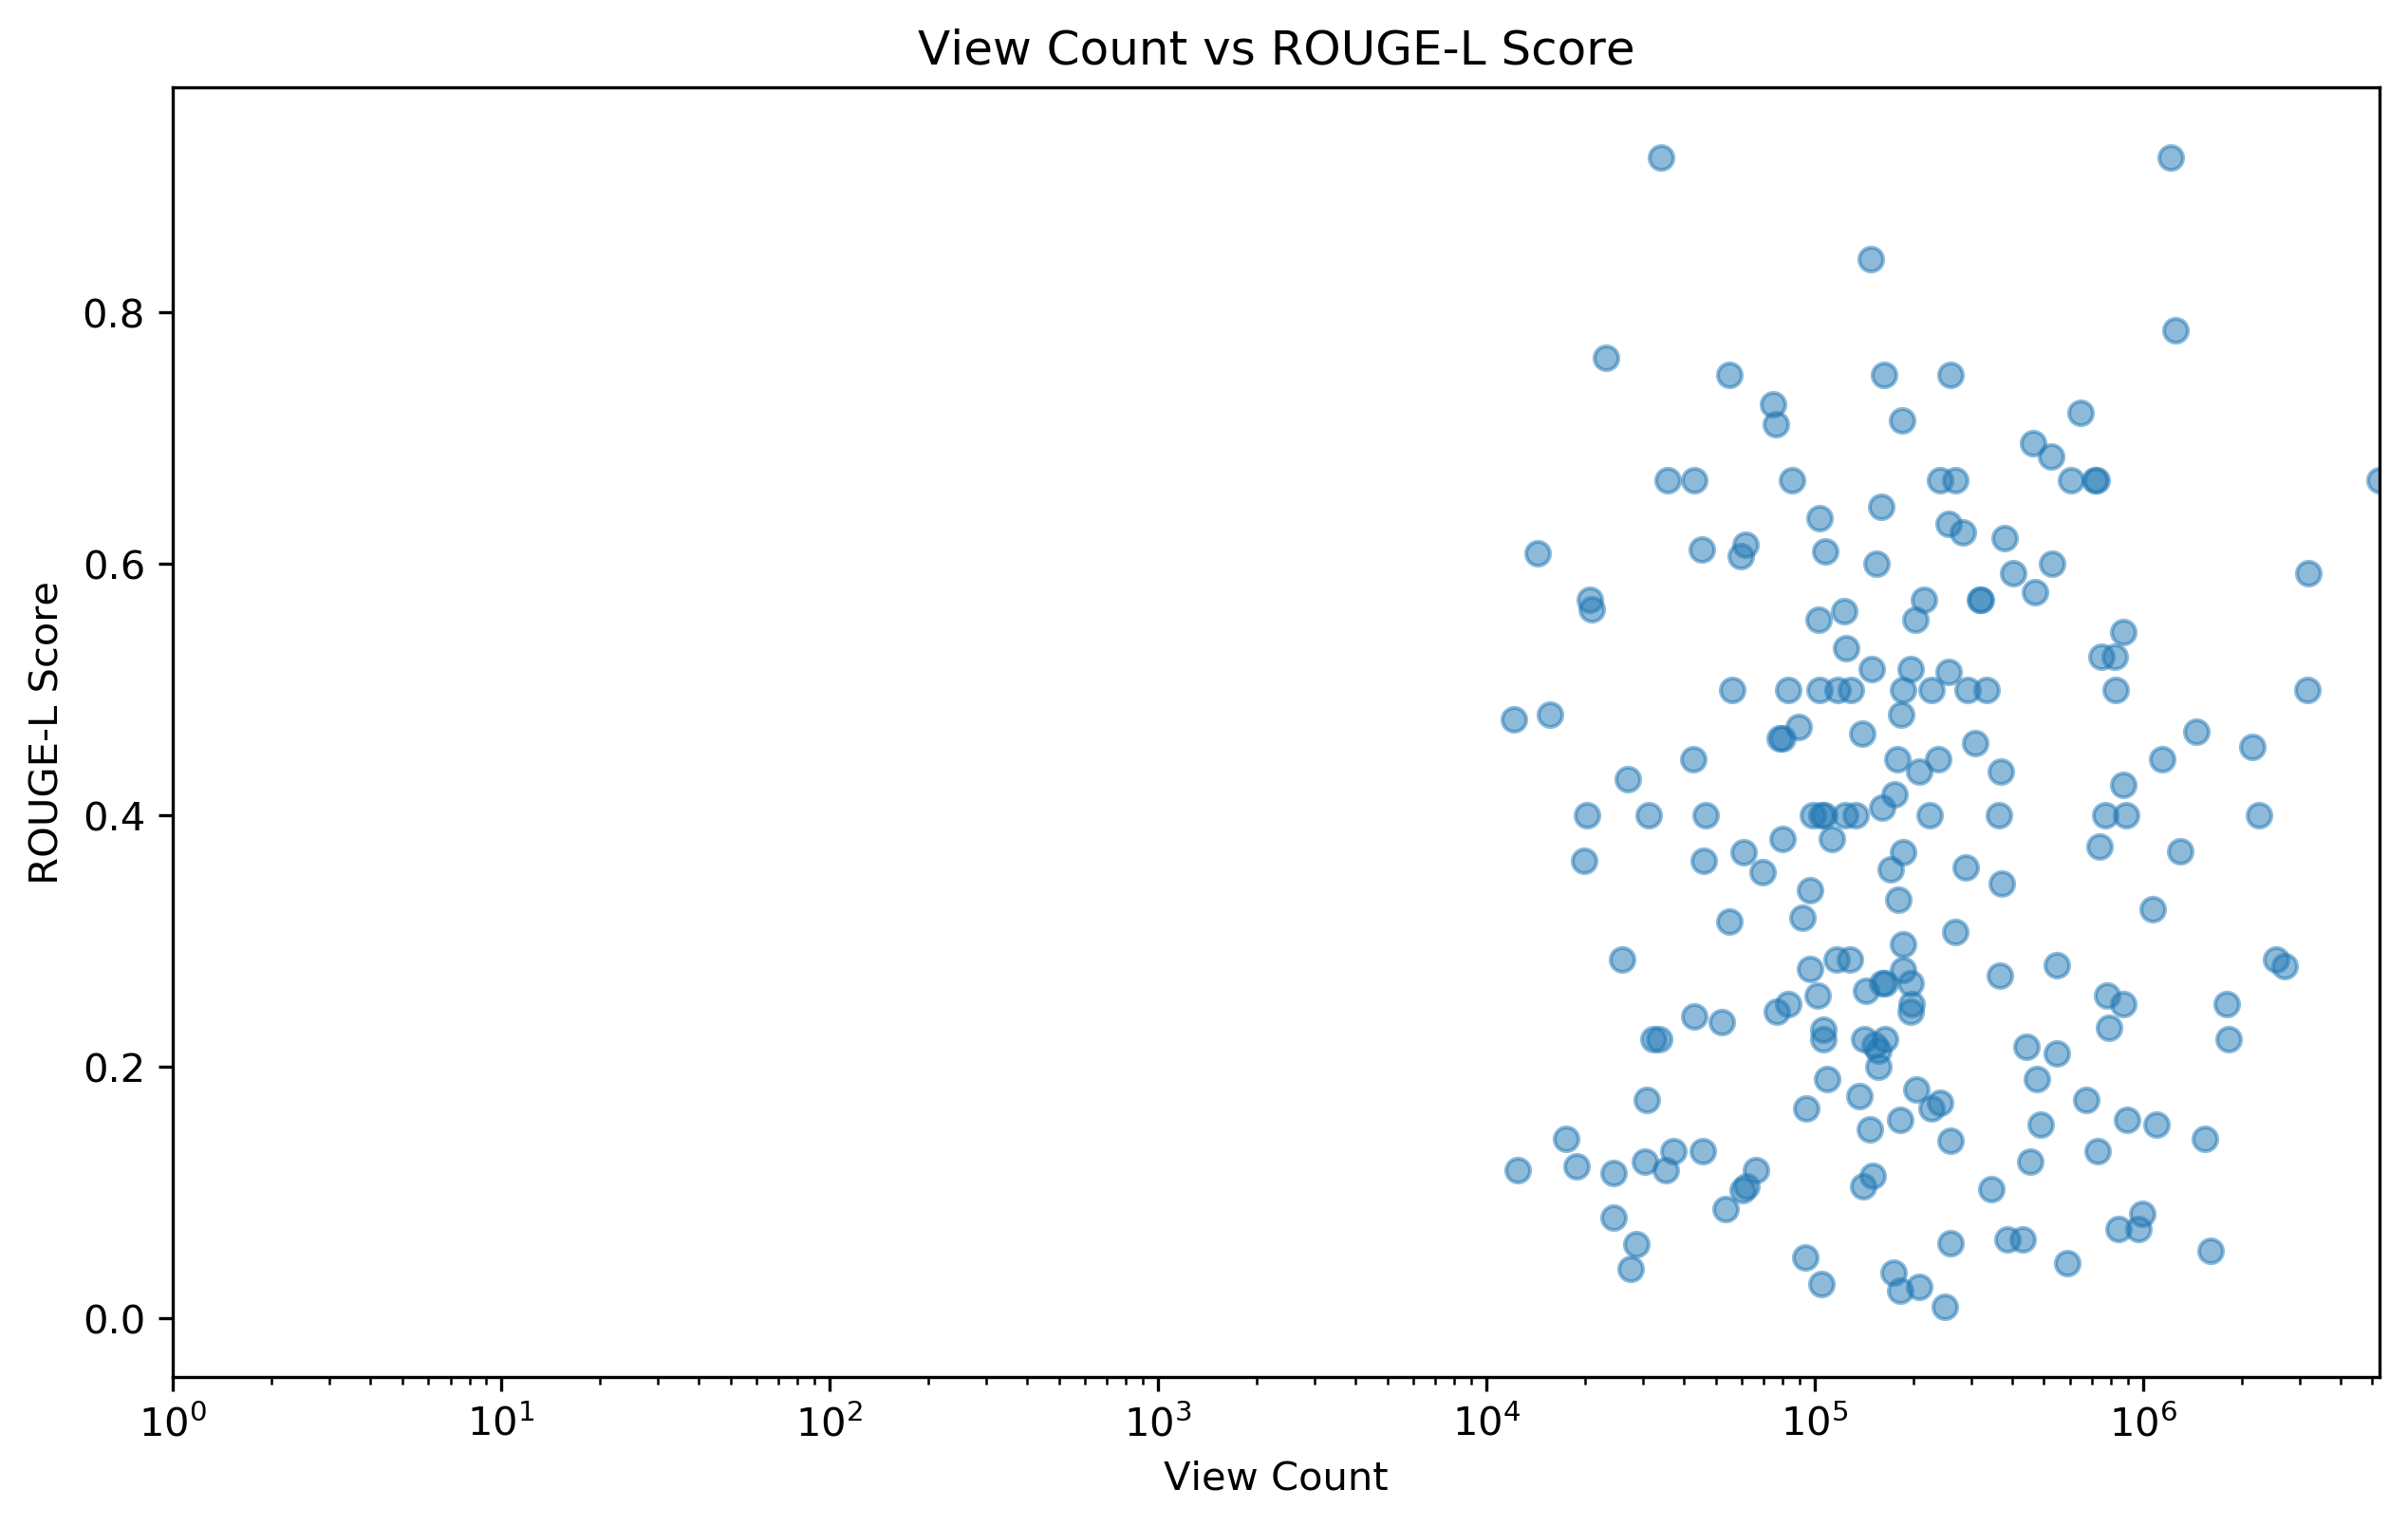
\includegraphics[width=0.65\textwidth]{../results/img/view_count_vs_rouge_score.png}
  \caption{再生回数とROUGE-Lスコアの関係}
\end{figure}

\subsection{動画の長さとROUGE-Lスコアの関係}
動画の長さとROUGE-Lスコアの間には弱い負の相関が見られた(Spearman's rank correlation:-0.19)。

\begin{figure}[htbp]
  \centering
  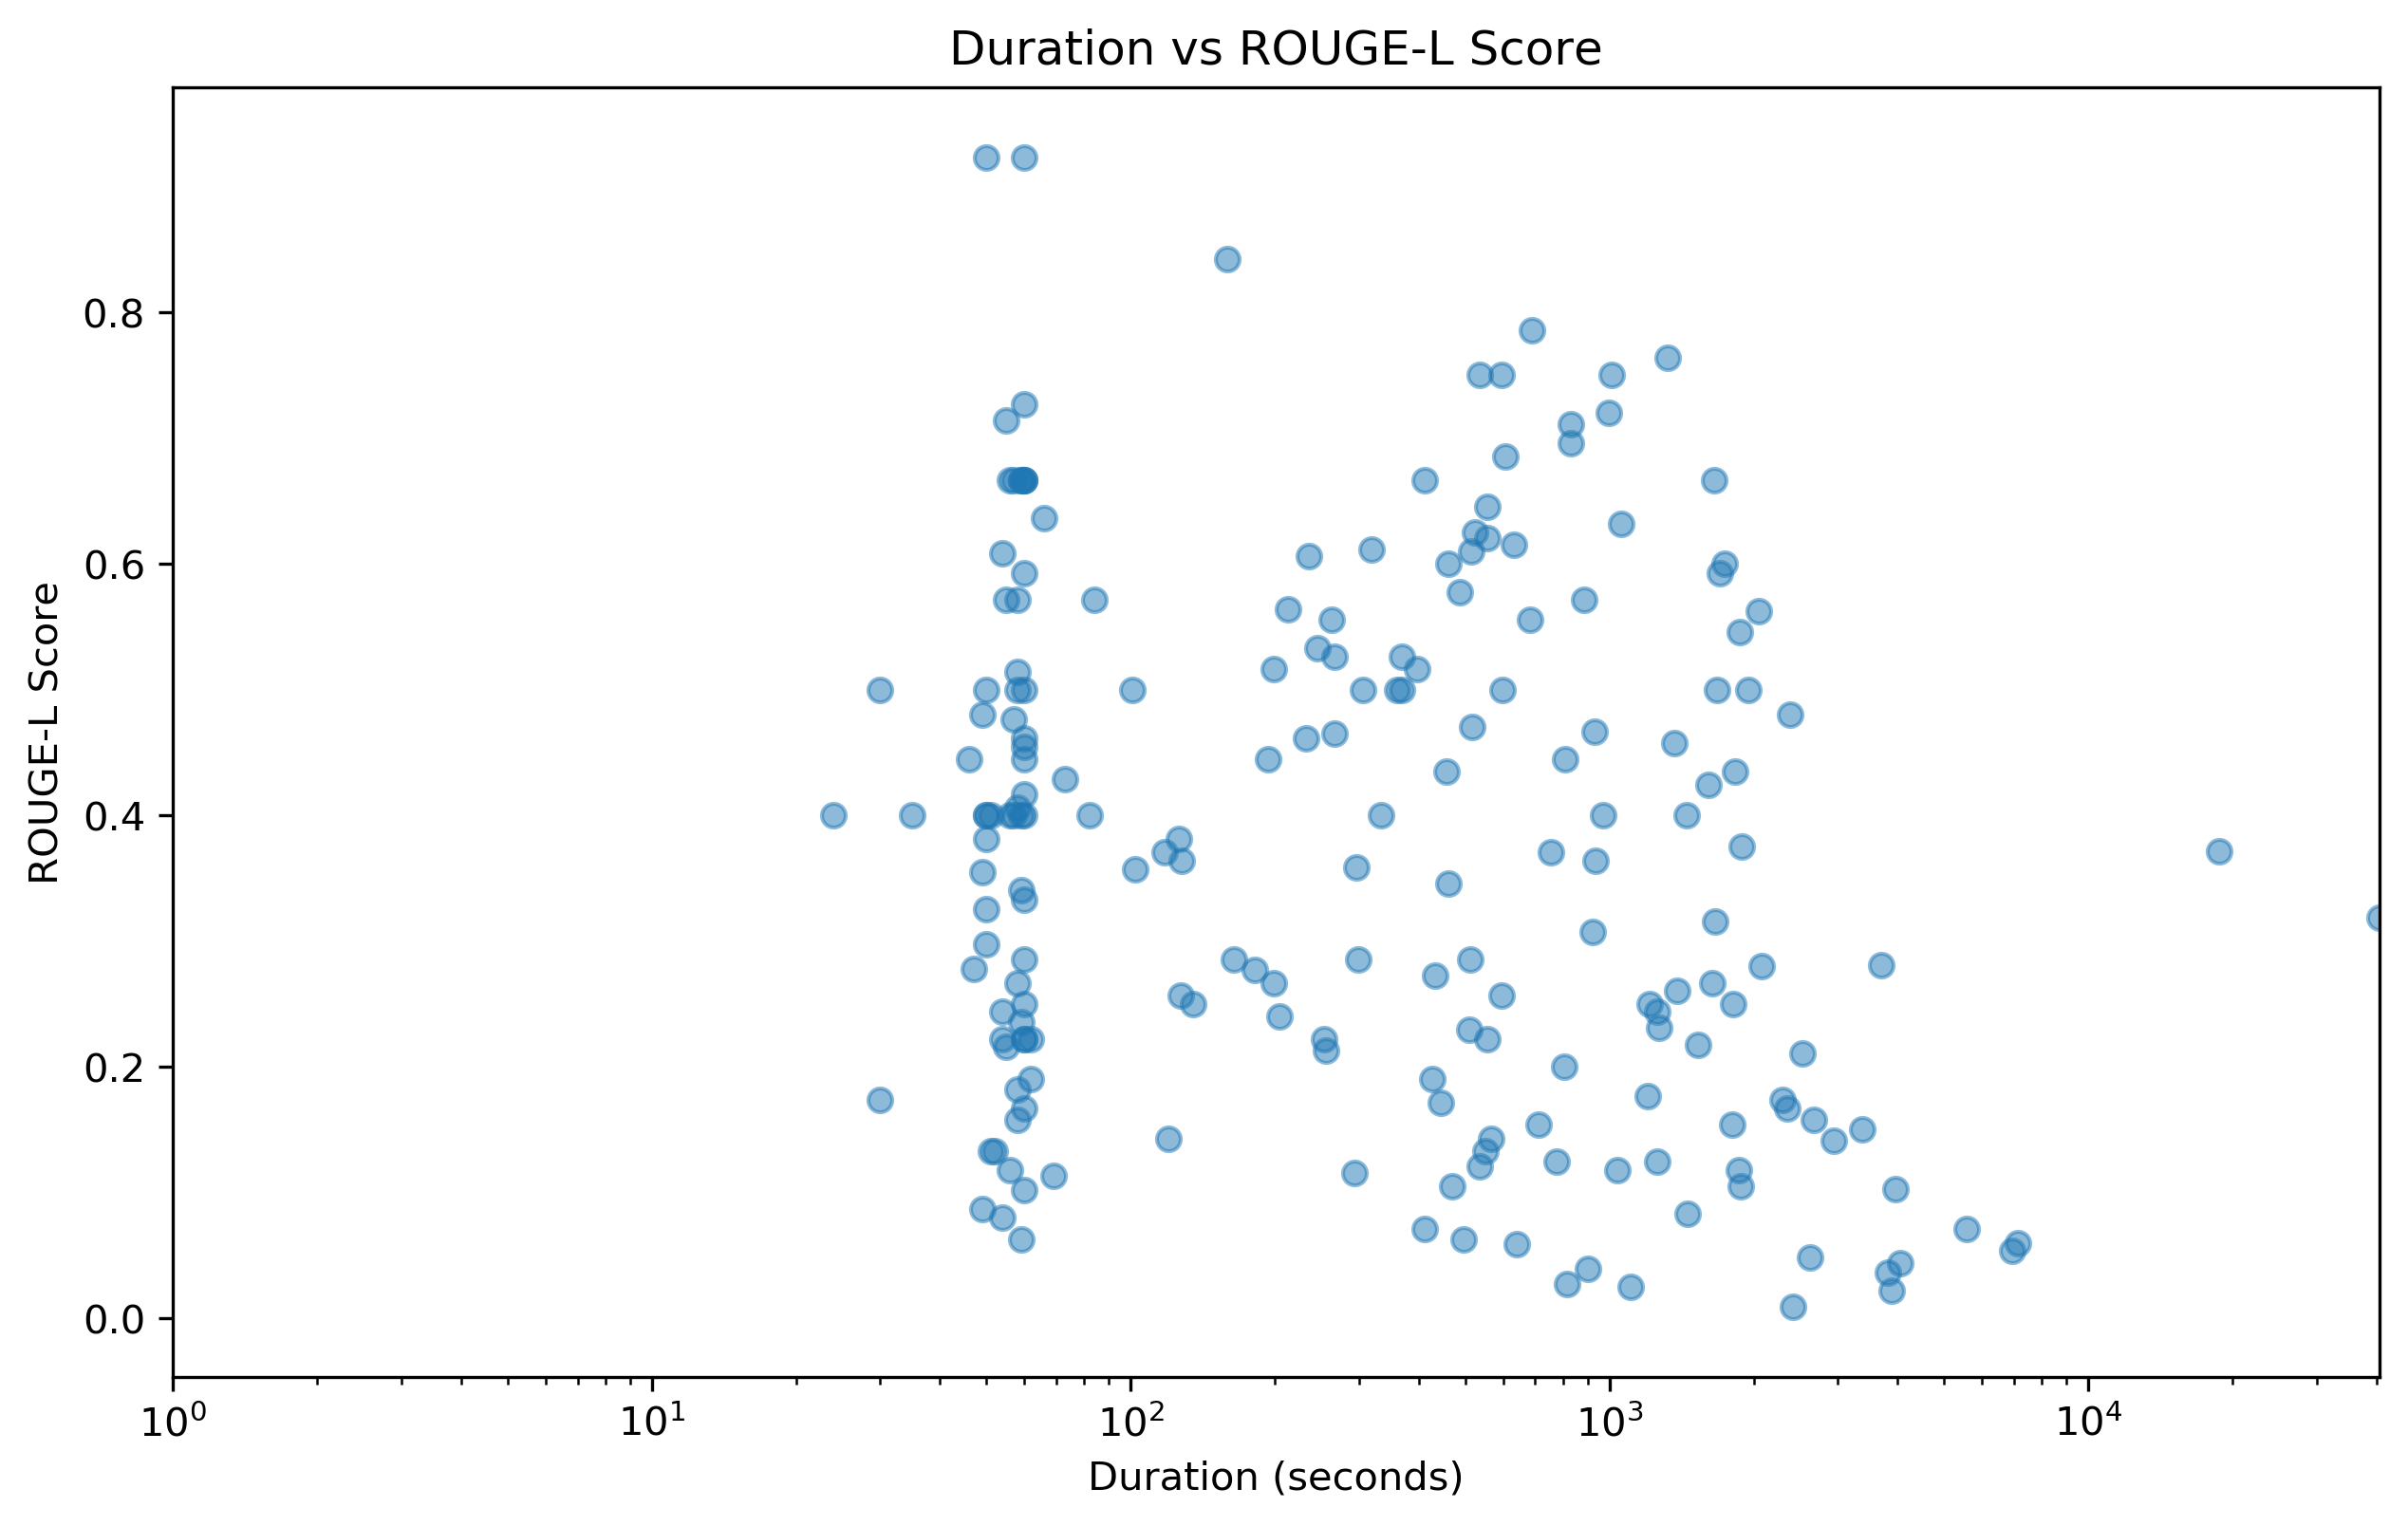
\includegraphics[width=0.65\textwidth]{../results/img/duration_vs_rouge_score.png}
  \caption{動画の長さとROUGE-Lスコアの関係}
\end{figure}

\subsection{チャンネル別の分析}
チャンネル間で字幕の品質に差があることが明らかになった。

\begin{figure}[htbp]
  \centering
  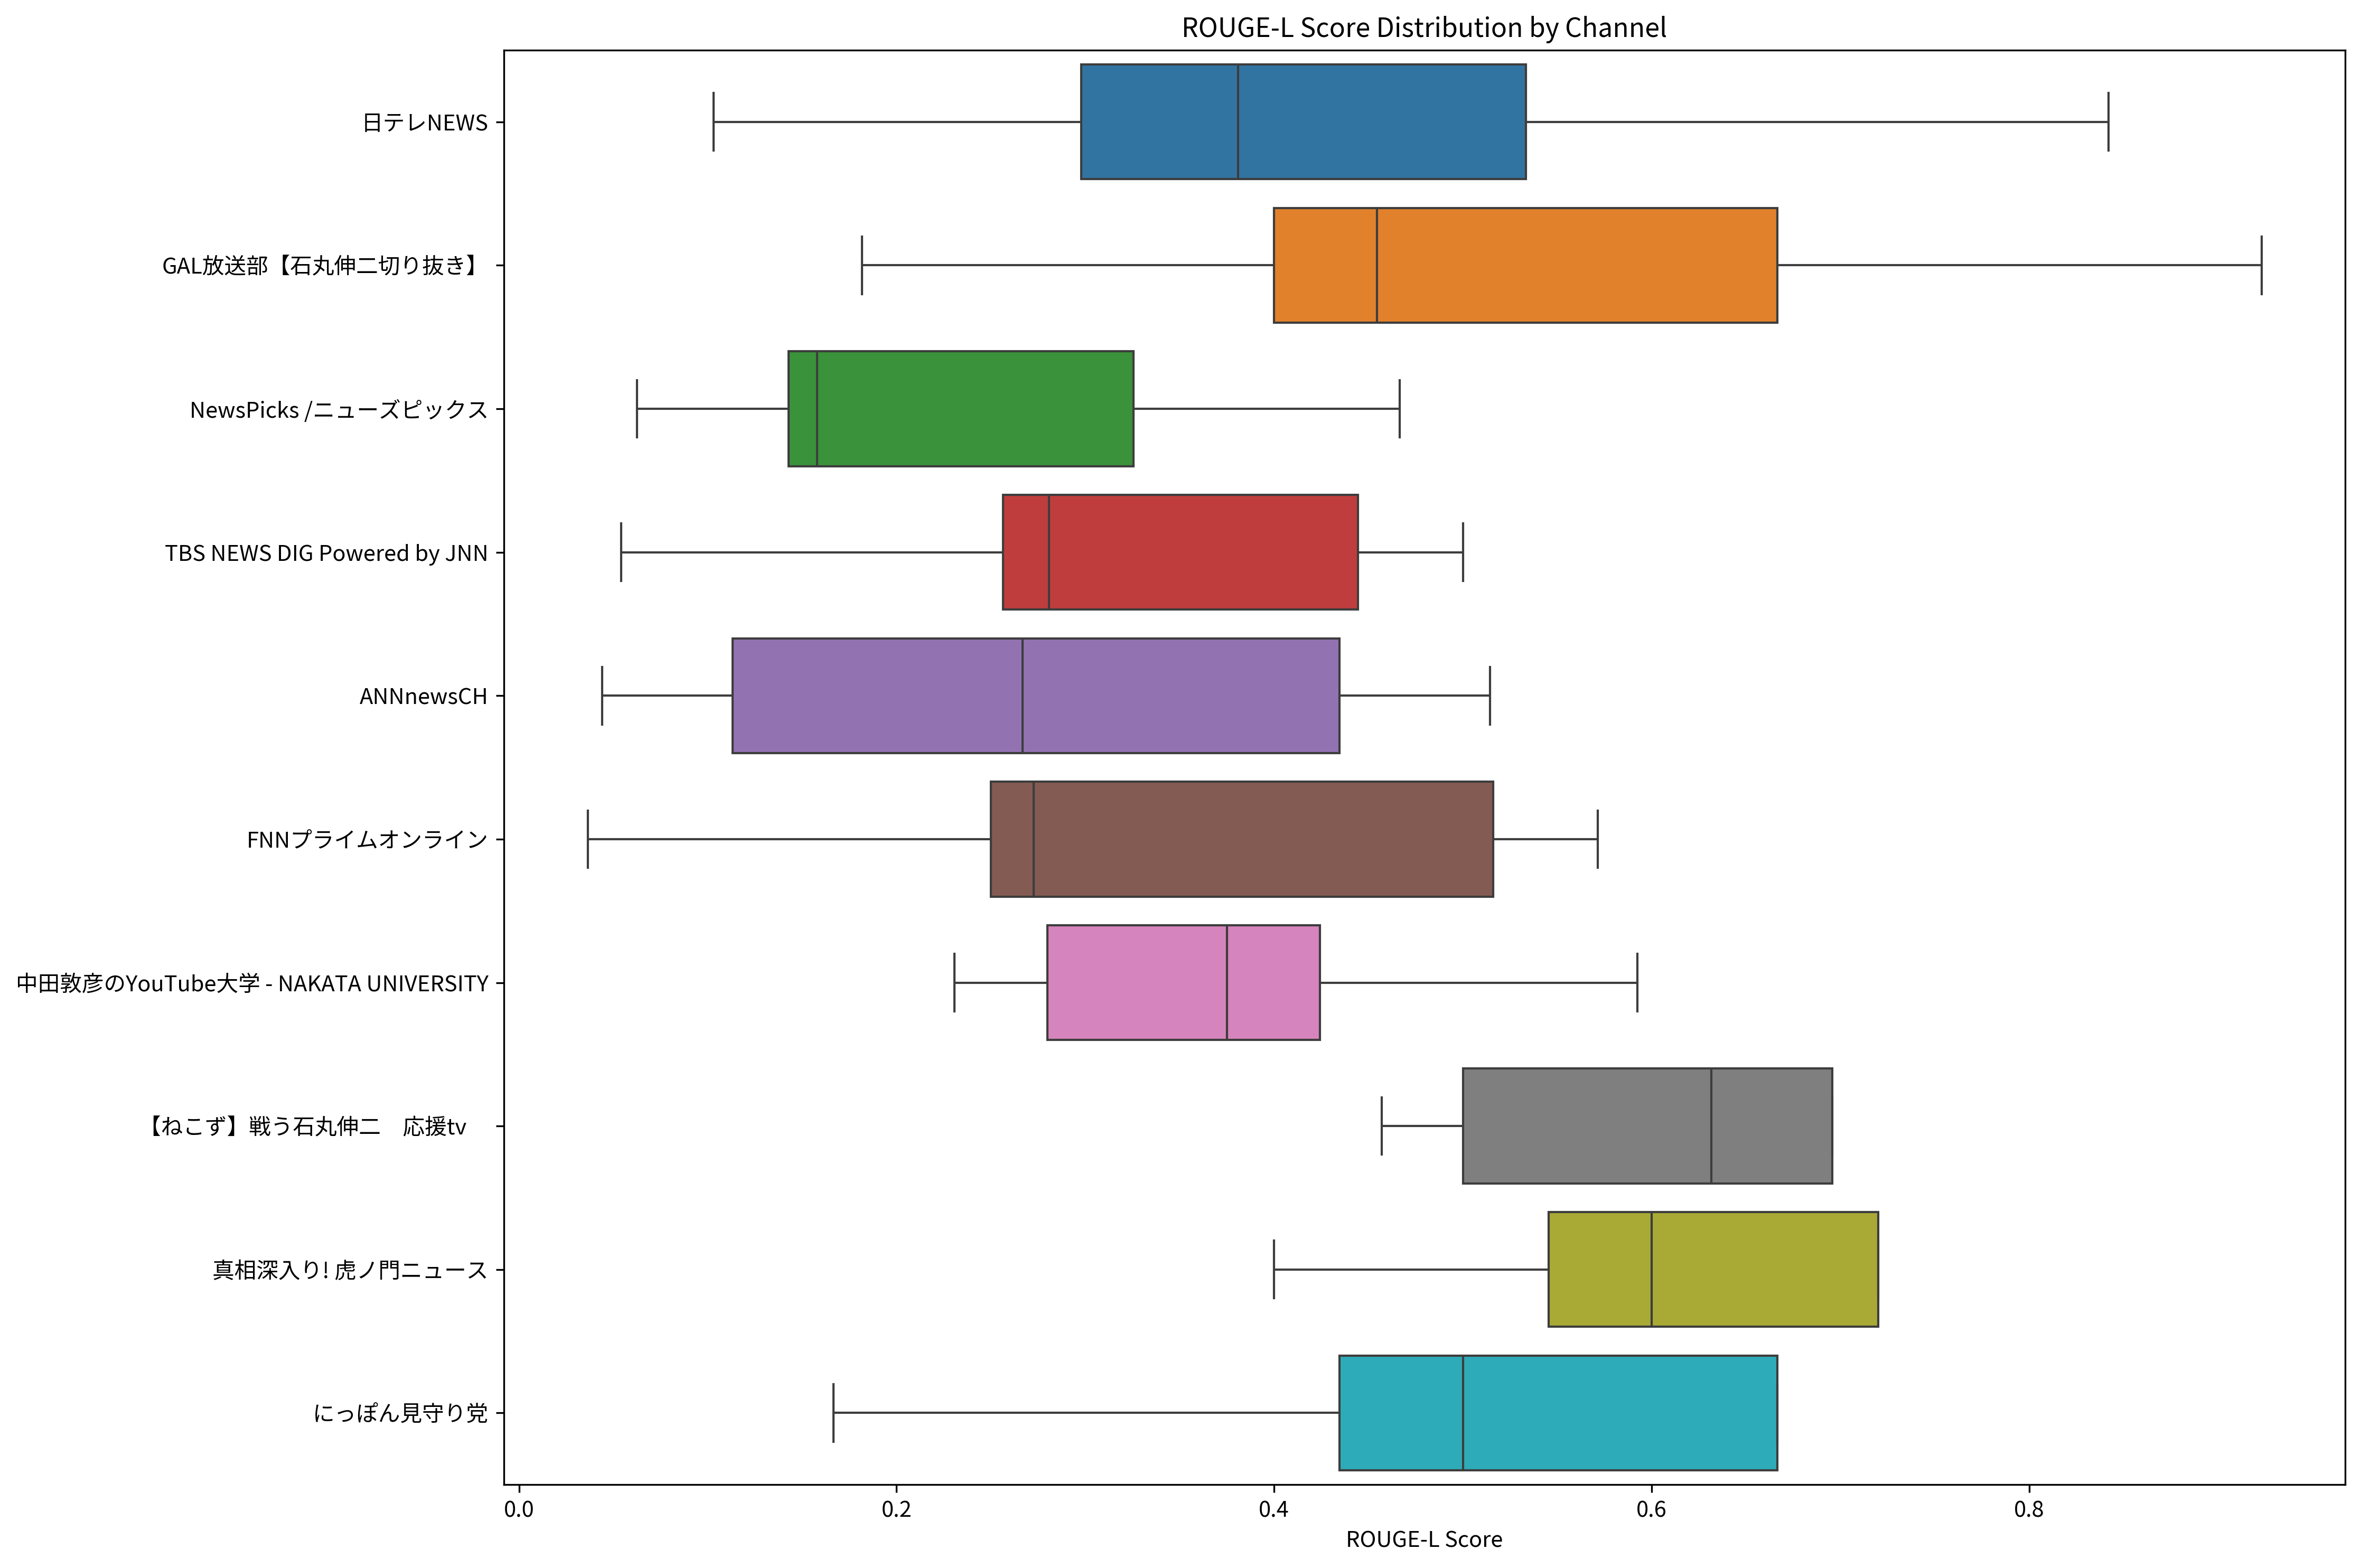
\includegraphics[width=0.65\textwidth]{../results/img/rouge_l_boxplot_by_channel.png}
  \caption{主要10チャンネルのROUGE-Lスコア分布}
\end{figure}

\section{結論}
本プロジェクトでは、YouTubeの動画分析ツールを実装し、500本の実際の動画データを用いて評価を行った。得られた主な結果は以下の通りである:

\begin{itemize}
  \item ショート動画の方が通常動画よりもROUGE-Lスコアが高い傾向が見られた。これは、ショート動画の方が手動で字幕を付ける手間が少なく、付与されにくいことを示唆している可能性がある。
  \item 動画の長さと字幕品質には弱い負の相関が見られた。これは、動画が長くなるほど字幕の品質が若干低下する傾向があることを示唆している。
  \item 再生回数と字幕品質にはほとんど相関が見られなかった。これは、動画の人気度と字幕の品質には直接的な関連がない可能性を示している。
  \item チャンネルによって字幕の品質に大きな差があることが明らかになった。これは、チャンネルごとの字幕生成や管理方針の違いを反映している可能性がある。
\end{itemize}

今後の課題としては、より多様なジャンルの動画での評価、言語別の分析、時系列での字幕品質の変化の追跡などが挙げられる。本研究の成果は、動画コンテンツの品質向上、自動字幕生成システムの改善、効果的な動画マーケティング戦略の立案など、様々な分野での応用が期待できる。

\end{document}